\section{Temperature sweeps}

Figure~\ref{Fig:ResH:TSweeps} shows the in-plane resistivity, $\rho(T)$ for each of the samples in zero field taken in the \ac{VTI} in the Polo magnet. From this plot we can characterise the \Tc of the samples and find the residual resistivity, $\rho_0$ by using simple linear fits to the data above the transition temperatures and extrapolate back to zero. Table~\ref{Table:ResH:TSweepFitsParams} show the fit parameters for each of the samples. 
\begin{table}
	\begin{center}
       	\caption{Fits parameters to $\rho = \rho_0 + \rho_1T$ for zero field resistivity data above $T_c$ as well as $T_c$ values determined from the same plots. Fits at low $T$ are shown in inset to figure~\ref{Fig:ResH:TSweeps}.}
		{\small \begin{tabular}[htbp]{lrrrr}
\toprule
Sample		& $\rho_0 (\unit{\micro\ohm\centi\metre})$	& $\rho_1 (\unit{\micro\ohm\centi\metre})$  & $T_c$ (\unit{\kelvin})	& $T_c/T_c(\textrm{max})$	\\
\midrule
B00KOD1A	& 40.7		& 0.454     & $0\pm1.0$	    & $0.00\pm0.03$	\\
B07KOD2		& 73.0		& 1.026     & $11\pm3.8$	& $0.31\pm0.11$	\\
B16KOD1A	& 49.9		& 0.843     & $17\pm1.0$	& $0.47\pm0.03$	\\
B30KOD3		& 15.9		& 0.578     & $29\pm0.5$	& $0.81\pm0.01$	\\
B32KOP1		& 54.2		& 0.824     & $36\pm1.0$	& $1.00\pm0.03$	\\
B32KOP4		& 55.6		& 1.904     & $35\pm2.0$	& $0.97\pm0.06$	\\
B30KUD3		& 123.0		& 2.233     & $32\pm1.0$	& $0.89\pm0.03$ \\
B28KUD3A	& 22.6		& 0.806     & $32\pm1.0$	& $0.89\pm0.03$	\\
\bottomrule
		\label{Table:ResH:TSweepFitsParams}
		\end{tabular} }
	\end{center}
\end{table}
The residual resistivities are very good with only one being above \unit{100}{\micro\ohm\centi\metre} and most below \unit{70}{\micro\ohm\centi\metre} which has been cited as being exceptionally good for \ac{BSCO}~\cite{Ando1999}. Moreover the \Tc of the optimally doped sample is \unit{36}{\kelvin} which is amongst the highest reported~\cite{Ando1999} which again is testament to the crystal quality. $\rho_0$ generally increases as you move away from critical doping which lends support to the notion of the La doping increasing the disorder in the CuO layers.

The inset to figure~\ref{Fig:ResH:TSweeps} shows the $\rho(\unit{300}{\kelvin})$ values for the samples along with error bars due to uncertainty in the size determination. As we saw in the previous section, there is significant misalignment and overall width to the voltage contacts which lead to large systematic errors which affect scaling only. Nonetheless, there appears to be an downward trend in resistivity as doping is increased. The circled points are B30KUD3 in both the overdoped and underdoped position and although the position is perhaps more fitting in the underdoped position, there error bars leave the overdoped point well within the overall trend.


% \begin{table}
% 	\begin{center}
%        	\caption{Fits parameters to $\rho = \rho_0 + \alpha_1T +
%        	\alpha_2T^2$ for zero field resistivity data above $T_c$.
%        	Fits at low $T$ are shown in inset to figure~\ref{Fig:ResH:TSweeps}}
% 		\begin{tabular}[htbp]{lrrr}
% \toprule
% Sample		& $\rho_0 (\times10^-2)$	& $\alpha_1 (\times10^{-4})$	& $\alpha_2 (\times10^{-7})$	\\
% \midrule
% B00KOD1A	& 12.26		& 6.895		& 14.394		\\
% B07KOD2		& 9.03		& 7.740		& 8.459			\\
% B16KOD1a	& 4.25		& 4.809		& 3.610			\\
% B30KOD3		& 1.43		& 3.385		& 4.595			\\
% B32KOP1		& 1.20		& 2.596		& -0.810		\\
% B32KOP4		& 2.76		& 21.886	& -8.862		\\
% B30KUD3		& 18.80		& 38.028	& -4.385		\\
% B28KUD3a	& 2.71		& 18.447	& -6.756		\\
% \bottomrule
% 		\label{Table:ResH:TSweepFitsParams}
% 		\end{tabular}
% 	\end{center}
% \end{table}


\section{Hall plots}

Figures~\ref{Fig:ResH:HallIndividualOD}, \ref{Fig:ResH:HallIndividualOP} and \ref{Fig:ResH:HallIndividualUD} show the Hall coefficients extracted as described in the methods section for samples progressing from overdoped, optimally doped to underdoped respectively. Where appropriate, the data is compared to that from Ando \etal~\cite{Ando1999}. Red lines in the plots are guides to the eye.

For the samples of $T_C >= \unit{28}{\kelvin}$ there are some data which did not reach sufficient field to obtain linear behaviour which are circled with a dashed line in the plots. For sample B30KOD2, many of the sweeps for $T < \unit{45}{\celsius}$ showed significant hysteresis due to temperature drift. Despite temperature correction, many of the fits did not pass through the origin (circled in the figure) which is a good indicator that the true field suppressed linear Hall has not been obtained. The same goes for the circled points on the B30KUD2 plot and another data point at $T=\unit{1.5}{\kelvin}$ and $R_H = \unit{$7.3\times10^{-3}$}{\centi\metre\cubed}$ from the first trip to \ac{LNCMI} which is outside the plot boundary as well as data points on the plot for B28KUD3B. The data sets are combined, minus the points highlighted in the previous paragraph, in the main panels of figure~\ref{Fig:ResH:InvHallCombined} alongside the data from the Ando paper.

\begin{figure}[htbp]
	\begin{center}
		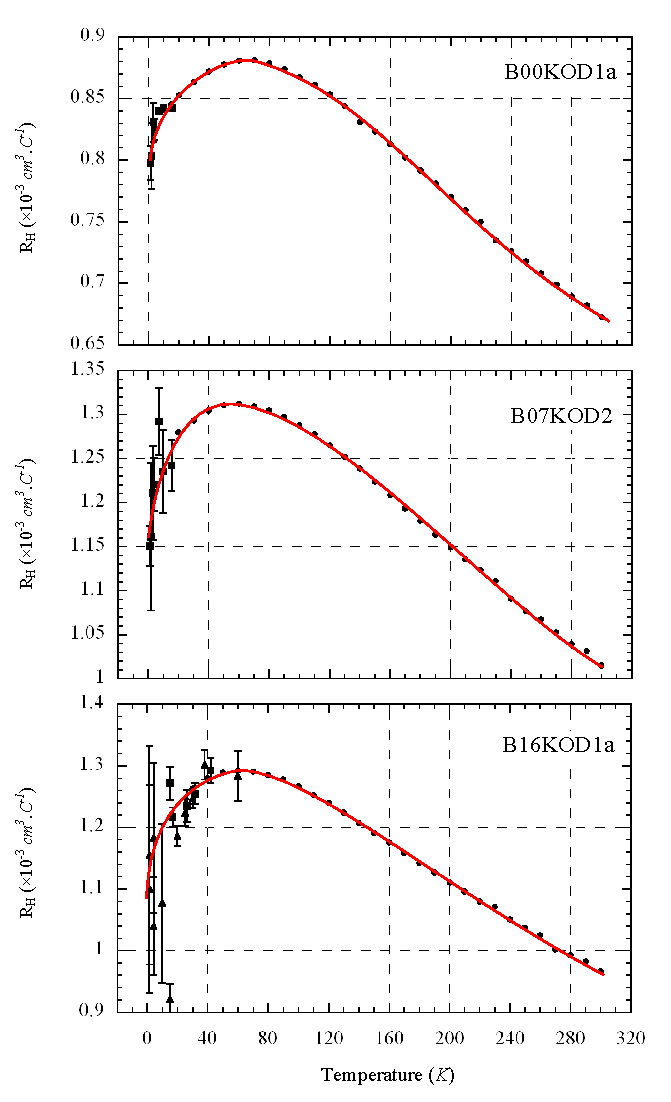
\includegraphics[scale=0.9]{Chapter-HallBSCO/Figures/HallIndividual/HallIndividualOD}
		\caption{$R_H$ for underdoped samples of \ac{BSCO}. Plots show results from, $\bullet$ Polo in June 2010, $\blacktriangle$ \ac{LNCMI} in June 2009, $\blacktriangledown$ \ac{LNCMI} in Feb 2010, $\blacksquare$ Nijmegen in May 2010. Symbols for comparable samples are marked on the plots. Red lines are a guide to the eye.}
		\label{Fig:ResH:HallIndividualOD}
	\end{center}
\end{figure}

\begin{figure}[htbp]
	\begin{center}
		\includegraphics[scale=0.9]{Chapter-HallBSCO/Figures/HallIndividual/HallIndividualOP}
		\caption{$R_H$ for underdoped samples of \ac{BSCO}. Plots show results from, $\bullet$ Polo in June 2010, $\blacktriangle$ \ac{LNCMI} in June 2009, $\blacktriangledown$ \ac{LNCMI} in Feb 2010, $\blacksquare$ Nijmegen in May 2010. Symbols for comparable samples are marked on the plots. Dashed lines indicate points where the field was not sufficient to achieve linear behaviour. Red lines are a guide to the eye.}
		\label{Fig:ResH:HallIndividualOP}
	\end{center}
\end{figure}

\begin{figure}[htbp]
	\begin{center}
		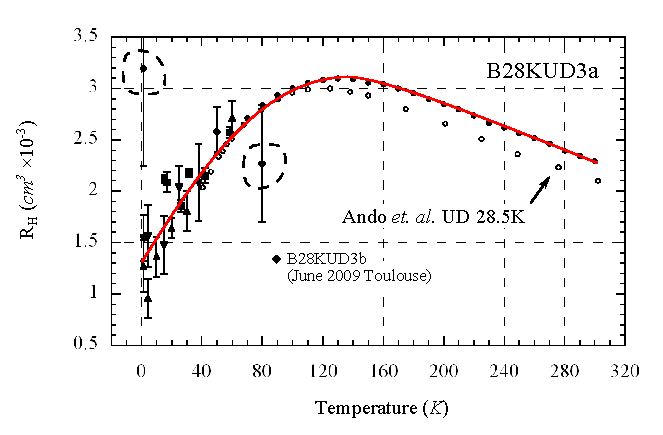
\includegraphics[scale=0.9]{Chapter-HallBSCO/Figures/HallIndividual/HallIndividualUD}
		\caption{$R_H$ for underdoped samples of \ac{BSCO}. Plots show results from, $\bullet$ Polo in June 2010, $\blacktriangle$ \ac{LNCMI} in June 2009, $\blacktriangledown$ \ac{LNCMI} in Feb 2010, $\blacksquare$ Nijmegen in May 2010. Symbols for comparable samples are marked on the plots. Dashed lines indicate points where the field was not sufficient to achieve linear behaviour. Red lines are a guide to the eye.}
		\label{Fig:ResH:HallIndividualUD}
	\end{center}
\end{figure}
\begin{figure}[htbp]
	\begin{center}
		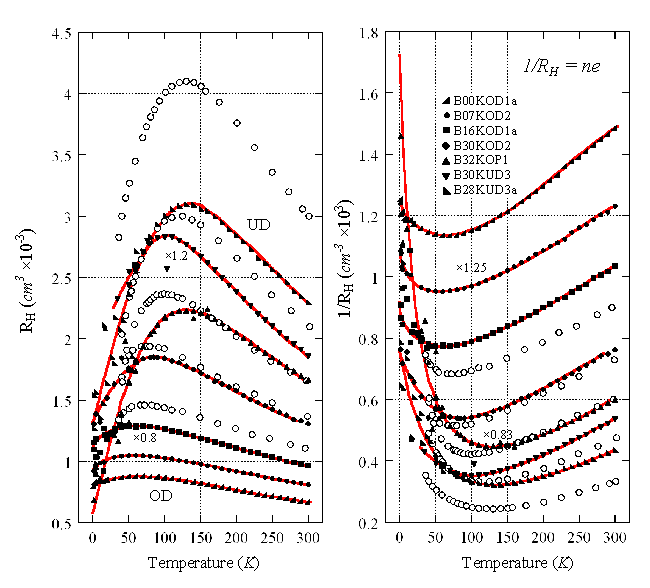
\includegraphics[scale=1.1]{Chapter-HallBSCO/Figures/InvHallCombined/InvHallCombined}
		\caption{Hall data in context with data from Ando \etal\cite{Ando1999} (open circles) which are in order of increasing $R_H$, 24KOD, 30KOD, 33KOP, 28.5KUD, 20KUD. Right panel shows the inverse hall data which relates to carrier density. Red lines are the same guides to the eye used in previous figures. Inset shows $R_H$ at \unit{300}{\kelvin} plus systematic error bars due primarily to uncertainty in thickness vs. doping scaled to \ac{TL2201} data. B30KUD3 (circled) is plotted in both the overdoped and underdoped positions.}
		\label{Fig:ResH:InvHallCombined}
	\end{center}
\end{figure}

With reference to figure~\ref{Fig:ResH:InvHallCombined} and in particular the new low temperature data points, we see that doping strongly affects the qualitative shape of the $R_H$ curves. Whilst the trend appears to be that $R_H(\unit{300}{\kelvin})$ decreases as doping increases as to be expected, the $R_H(\unit{0}{\kelvin})$ values all tend toward approximately similar values of around \unit{$0.5\times 10^{-3}$}{\centi\metre\cubed}to \unit{$1.5\times 10^{-3}$}{\centi\metre\cubed}. The most pronounced difference between high and low temperature values though is with the optimally doped samples which are around $\times 2.75$ greater at high temperature. Right down to \unit{0}{\kelvin} there is no sign change in $R_H$, which suggests that the hole pockets have higher mobility than the electron pockets across the range of dopings studied.

The error bars on the data points do not include error from the thicknesses which are systematic across the data points. The inset of figure~\ref{Fig:ResH:InvHallCombined} shows the $R_H$ values at \unit{300}{\kelvin} vs. doping for each of the samples with these error bars applied. The overall trend is downward with doping with the progression being approximately monotonic, however the exception is B16KOD1A which has a slightly lower $R_H$ than would be expected from a linear trend.

The Hall angle is plotted for each of the samples where $B=\unit{0}{\tesla}$ in-plane resistivity data is available in figure~\ref{Fig:ResH:HallAngle} with temperature raised to a fitted exponent, $\alpha$. In the original Chien analysis, $\alpha = 2$ but is allowed to vary here to observe deviations from the expected $T^2$ behaviour. Similar analysis was performed for resistivity data taken at $B=\unit{13}{\kelvin}$ and although these plots are not shown, the fitted $\alpha$ values are plotted in the bottom left subplot along with the $B=\unit{0}{\tesla}$ values. A nominal unitary field was used when calculating $\cot\theta_H$ and only data above the superconducting transition was fitted and is shown in the plots. Note that for the $B=\unit{13}{\tesla}$ case, the Hall data for the optimally doped sample B32KOP1 was compared with resistivity data for sample B32KOP4 which explains the slightly different doping value assigned to it. In this particular instance, it appears that the assignment of the sample B30KUD3 would be more suited to underdoped rather than overdoped.

\begin{figure}[htbp]
    \begin{center}
        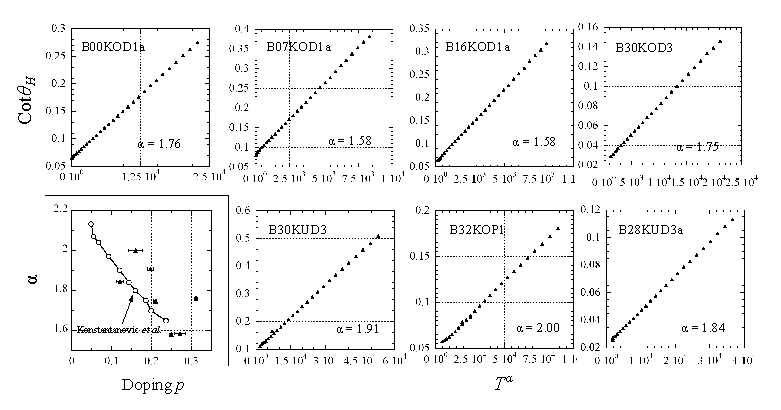
\includegraphics[scale=1.1]{Chapter-HallBSCO/Figures/HallAngle/HallAngle}
        \caption{Hall angle calculated with a nominal field of unity from resistivity data taken in zero field. Plot in bottom left shows the fitted exponent, $\alpha$, vs. doping compared with similar data on \ac{BSCO} from Konstantanovi\'c \etal~\cite{Konstantinovic2000} for both zero field resistivity data and resistivity data taken at \unit{13}{\kelvin} ($\cot\theta_H$ plots for $B=\unit{13}{\tesla}$ not shown)}
        \label{Fig:ResH:HallAngle}
    \end{center}
\end{figure}
With reference to the plot in the lower left, the fitted exponents approximately follow the same downward trend with doping as in \ac{BSCO} data from Konstantanovi\'c \etal~\cite{Konstantinovic2000} up to around $p=0.27$. In particular the $B=\unit{13}{\tesla}$ follows the curve reasonably closely before the upturn at $p=0.31$. Downward deviation from the $T^2$ behaviour at high temperatures (as indicated from a drop in the $\alpha$ exponent) at this point in the phase diagram has been previously interpreted to be due to the saddle point in the \ac{DOS} which is approaching from below the Fermi energy~\cite{Ando2004} which would also explain why there is a recovery toward $T^2$ behaviour between $p=0.27$ and $p=0.31$ as the flat portion of the \ac{DOS} passes above the Fermi energy. This would suggest that the van-Hove singularity peaks in the \ac{BSCO} phase diagram at around $p=0.25$, approximately where the B16KOD1A sample lies and where the room temperature $R_H$ value was also found to be slightly lower than expected. However this occurs at a higher doping than the Hashimoto paper would suggest~\cite{Hashimoto2008} (see figure~\ref{Fig:Intro:VanHoveBSCOLSCO}) and given the proximity of the van-Hove singularity, the low Hall coefficient should not be interpreted a simple indicator of carrier density. 
\begin{figure}[htbp]
    \begin{center}
        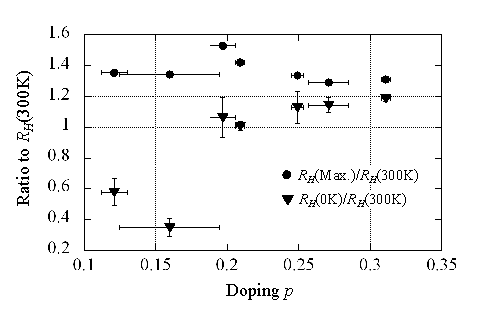
\includegraphics[scale=0.8]{Chapter-HallBSCO/Figures/RhRatios/RhRatios}
        \caption{Left shows ratio of $R_H$ values at the maximum of the Hall curves and at $T=\unit{0}{\kelvin}$ to the $T=\unit{300}{\kelvin}$ $R_H$ values. Errors in $R_H(\unit{0}{\kelvin}$ estimated from Hall plots, the value for B30KUD2 is estimated based on linear extrapolation. Right shows the temperature where the maximum $R_H$ occurs.}
        \label{Fig:ResH:RhRatios}
    \end{center}
\end{figure}

An alternate explanation based on the Narduzzo paper~\cite{Narduzzo2008} goes as follows. For $p \gtrsim 0.19$, $R_H(\unit{0}{\kelvin}) > R_H(\unit{300}{\kelvin})$ as illustrated in figure~\ref{Fig:ResH:RhRatios}. If we assume there is not temperature dependent change of the Fermi surface such that would affect $\vect{v_F}$, then this can be explained by an temperature dependent change in scattering that preferentially affects one of the two regions of curvature (hole-like or electron-like) on the Fermi surface i.e. a change in anisotropic scattering. As detailed in the introduction, such scattering is thought to originate in the overdoped side of the phase diagram and is seemingly closely tied to superconductivity. The Narduzzo paper explores this possibility but ultimately could not definitively conclude that the scattering rate is proportional to $\cos^2(2\phi)$ as is the case in the Abdel-Jawad paper~\cite{Abdel-Jawad2007} detailed in the introduction.

To explain the anisotropy in the van-Hove scenario where the change is thought to come about from a change in the carrier numbers, we must surmise that the flat band does not lie at the same energy all around the Fermi surface in order to achieve this anisotropy --- in effect this leads to a momentum dependent carrier term. This has been observed in cuprates with Plat\'e \etal~\cite{Plate2005} demonstrating in \ac{TL2201} a momentum dependence of the energy of the flat region of the bandstructure that range between \unit{-25}{\milli\electronvolt} and \unit{-40}{\milli\electronvolt}. However, along the $(\pi, \pi)$ direction in this case, the van-Hove peak was suppressed suggesting that scattering too is anisotropic.

When we consider the ratio of the maximum $R_H$ to the \unit{300}{\kelvin} value also plotted in figure~\ref{Fig:ResH:RhRatios} then we see that these values do not vary much at all with doping indicating that the scattering process that suppresses the low temperature Hall values only becomes dominant below the temperature where $R_H(\textrm{max})$ occurs. Moreover we note that the low temperature behaviour of $R_H$ which, although not possible to ascertain for certain due to the scatter in points, appears linear in temperature below $R_H(\textrm{max})$, which suggests that the same process explored above is $T$-linear in behaviour.

A finally observation is that when the temperatures of the maximums in $R_H$ are plotted in figure~\ref{Fig:ResH:RhRatios}, they show a similar doping behaviour to the $\alpha$ fitted exponents.




% There seems to be little evidence of the transition of the doping from $p$ to $1+p$ which agrees with the notion that these dopings lie beyond where the change in the size of the Fermi surface is thought to take place~\cite{LeBoeuf2007}. 

%Divergence in resistivity occurs beyond UD 0K\cite{Ando2000}, well
%below our lowest nominal doping of ...

% Residual resistivity of ~20\mu\Ohm cm at optimal doping is very small
% and increases with La doping i.e. as become more underdoped
% \cite{Ando2000}


